\documentclass[
  bibliography=totoc,     % Literatur im Inhaltsverzeichnis
  captions=tableheading,  % Tabellenüberschriften
  titlepage=firstiscover, % Titelseite ist Deckblatt
]{scrartcl}

% Paket float verbessern
\usepackage{scrhack}

% Warnung, falls nochmal kompiliert werden muss
\usepackage[aux]{rerunfilecheck}

% unverzichtbare Mathe-Befehle
\usepackage{amsmath}
% viele Mathe-Symbole
\usepackage{amssymb}
% Erweiterungen für amsmath
\usepackage{mathtools}

% Fonteinstellungen
\usepackage{fontspec}
% Latin Modern Fonts werden automatisch geladen
% Alternativ zum Beispiel:
%\setromanfont{Libertinus Serif}
%\setsansfont{Libertinus Sans}
%\setmonofont{Libertinus Mono}

% Wenn man andere Schriftarten gesetzt hat,
% sollte man das Seiten-Layout neu berechnen lassen
\recalctypearea{}

% deutsche Spracheinstellungen
\usepackage[ngerman]{babel}


\usepackage[
  math-style=ISO,    % ┐
  bold-style=ISO,    % │
  sans-style=italic, % │ ISO-Standard folgen
  nabla=upright,     % │
  partial=upright,   % │
  mathrm=sym,        % ┘
  warnings-off={           % ┐
    mathtools-colon,       % │ unnötige Warnungen ausschalten
    mathtools-overbracket, % │
  },                       % ┘
]{unicode-math}

% traditionelle Fonts für Mathematik
\setmathfont{Latin Modern Math}
% Alternativ zum Beispiel:
%\setmathfont{Libertinus Math}

\setmathfont{XITS Math}[range={scr, bfscr}]
\setmathfont{XITS Math}[range={cal, bfcal}, StylisticSet=1]

% Zahlen und Einheiten
\usepackage[
  locale=DE,                   % deutsche Einstellungen
  separate-uncertainty=true,   % immer Unsicherheit mit \pm
  per-mode=symbol-or-fraction, % / in inline math, fraction in display math
]{siunitx}

% chemische Formeln
\usepackage[
  version=4,
  math-greek=default, % ┐ mit unicode-math zusammenarbeiten
  text-greek=default, % ┘
]{mhchem}

% richtige Anführungszeichen
\usepackage[autostyle]{csquotes}

% schöne Brüche im Text
\usepackage{xfrac}

% Standardplatzierung für Floats einstellen
\usepackage{float}
\floatplacement{figure}{htbp}
\floatplacement{table}{htbp}

% Floats innerhalb einer Section halten
\usepackage[
  section, % Floats innerhalb der Section halten
  below,   % unterhalb der Section aber auf der selben Seite ist ok
]{placeins}

% Seite drehen für breite Tabellen: landscape Umgebung
\usepackage{pdflscape}

% Captions schöner machen.
\usepackage[
  labelfont=bf,        % Tabelle x: Abbildung y: ist jetzt fett
  font=small,          % Schrift etwas kleiner als Dokument
  width=0.9\textwidth, % maximale Breite einer Caption schmaler
]{caption}
% subfigure, subtable, subref
\usepackage{subcaption}

% Grafiken können eingebunden werden
\usepackage{graphicx}

% schöne Tabellen
\usepackage{tabularray}
\UseTblrLibrary{booktabs, siunitx}

% Verbesserungen am Schriftbild
\usepackage{microtype}

% Literaturverzeichnis
\usepackage[
  backend=biber,
]{biblatex}
% Quellendatenbank
\addbibresource{lit.bib}
\addbibresource{programme.bib}

% Hyperlinks im Dokument
\usepackage[
  german,
  unicode,        % Unicode in PDF-Attributen erlauben
  pdfusetitle,    % Titel, Autoren und Datum als PDF-Attribute
  pdfcreator={},  % ┐ PDF-Attribute säubern
  pdfproducer={}, % ┘
]{hyperref}
% erweiterte Bookmarks im PDF
\usepackage{bookmark}

% Trennung von Wörtern mit Strichen
\usepackage[shortcuts]{extdash}

\author{%
  Vincent Wirsdörfer\\%
  \href{mailto:vincent.wirsdoerfer@udo.edu}{authorA@udo.edu}%
  \and%
  Joris Daus\\%
  \href{mailto:joris.daus@udo.edu}{authorB@udo.edu}%
}
\publishers{TU Dortmund – Fakultät Physik}


\begin{document}

\section{Versuchsaufbau}
\label{sec:Versuchsaufbau}

\noindent Der allgemeine Versuchsaufbau wird in der untenstehenden Abbildung \ref{fig:Versuchsaufbau} dargestellt. Hauptbestandteil des Experiments
ist die Millikan-Kammer, welche den Kondensator mit Plattenabstand $d = \left(7.6250\pm0.0051\right)
\,\unit{\milli\meter}$ enthält. Die Öltröpfchen, welche ,durch eine Öffnung in der oberen Platte der Kammer,
in den Kondensator gelangen, besitzen eine Dichte von $\rho_\text{Oel}= 886\,\unit[per-mode=reciprocal]{\kilo\gram\per\cubic\meter}$ und 
werden durch eine Halogenlampe angestrahlt. Somit ist die Tröpfchenbewegung mittels des Mikroskops einfacher zu erkennen. Wie bereits 
in Kapitel \ref{sec:Theorie} erwähnt, sind die meisten Tröpfchen bereits durch Reibung elektrisch geladen. Falls dies 
jedoch vereinzelnd nicht der Fall ist, kann ggf. ein radioaktives Präparat angewendet werden, um die Ladung zu ändern.

\begin{figure}
    \centering 
    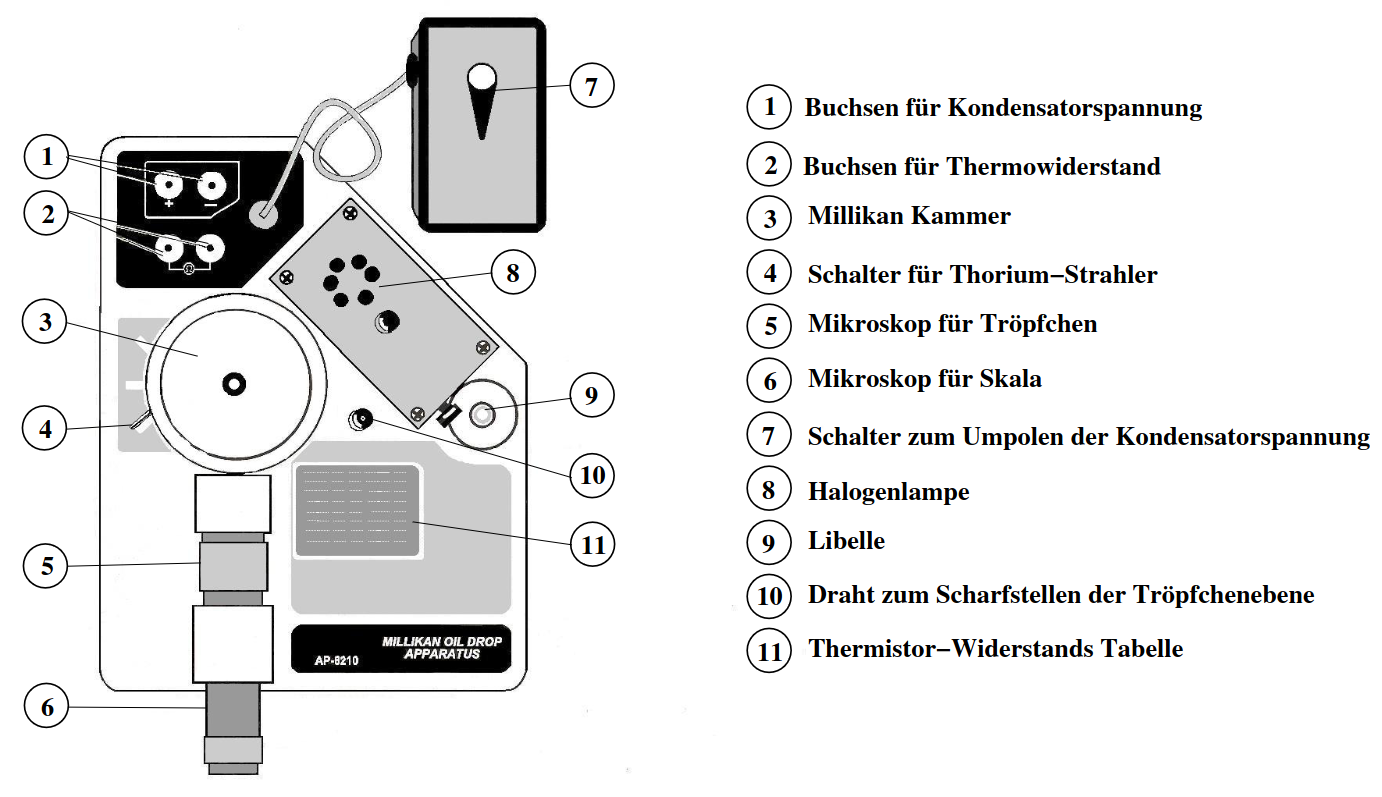
\includegraphics[height=6cm]{Aufbau.png}
    \caption{Experimenteller Versuchsaufbau des Millikan-Versuchs \cite{Versuchsanleitung_v503}.}
    \label{fig:Aufbau}
\end{figure}

\section{Versuchsdurchführung}
\label{sec:Versuchsdurchführung}

\noindent Vor Durchführung des Experiments wird mit Hilfe der Libelle die waagerechte Einstellung der Apparatur überprüft. Im 
Folgenden kann bei korrekter Anlegung der Spannungsquelle das E-Feld über einen Hebel aufgebaut werden. Zusätzlich wird sich mit 
dem Multimeter vertraut gemacht, welcher den Widerstand des Thermistors bei potentieller Erwärmung misst.\\

Im ersten Schritt des Versuchs werden die Öltröpfchen in das elektrische Feld des Kondensators zerstäubt. Im Rahmen der Zeitmessung 
müssen jedoch zunächst mehrere Einstellungen verändert werden, um die bestmögliche Betrachtungsperspektive gewährleisten zu 
können. Dazu zählt zum einen das Scharfstellen der Tröpfchenebene mit einem Draht wie in Abb. \ref{fig:Aufbau} beschrieben und zum
anderen die manuelle Anpassung des Mikroskops. Nachdem ein hinreichend langsames Tröpfchen gefunden wird, kann die Messung beginnen.
Hierzu wird eine geeignete Strecke auserkiesen, welche das Tröpfchen zurücklegt. Gleichzeitig wird die dafür benötigte Zeit gemessen
und das Experimentierheft übertragen, sodass die Geschwindigkeit ermittelt. Nach Überschreiten dieser Strecke werden die Platten
des Kondensators umgepolt, was dem Bewegungstrend des Tröpfchens entgegensetzt. Erneut wird für dieses spezielle Tröpfchen die für 
die Strecke benötigte Zeit gemessen und notiert. Dieser Vorgang wird so lange wiederholt bis maximal fünf Auf- und 
Abwärtsbewegungen betrachtet und gemessen werden. Zusätzlich wird nach jeder erfolgreichen Messung eines Tröpfchens der Widerstand 
des Thermistors abgelesen und aufgeschrieben.\\

\noindent Insgesamt werden die Geschwindigkeiten von 15 verschiedenen Tröpfchen genauer untersucht, welche zur Berechnung der
Elementarladung konsultiert werden können. Im Anschluss werden die Platten des Kondensators gesäubert und der Arbeitsplatz geordnet
hinterlassen.

\end{document}

